%=== INFO ======================================================================
% Author: Jamie Phan
%
%===============================================================================

%=== PACKAGES ==================================================================
    \documentclass[a4paper]{article}
    %Appearance
    \usepackage{microtype} %better typography
    \usepackage[english]{babel}
    \usepackage{fancyhdr} %for fancy page style
    \usepackage{color} %Added support for color text
        \definecolor{codegreen}{rgb}{0,0.6,0}
        \definecolor{codegray}{rgb}{0.5,0.5,0.5}
        \definecolor{codepurple}{rgb}{0.58,0,0.82}
        \definecolor{backcolour}{rgb}{0.95,0.95,0.92}

    %Document Dynamics
    \usepackage[colorlinks=true]{hyperref} %Manage links
    \hypersetup{linkcolor=blue}
    \usepackage{url}
    \usepackage{geometry} %For easy management of document margins
    \usepackage{graphicx} %Allows for insertion of images in document
    \graphicspath{ {figures/} {images/} }

    %Technical
    \usepackage{amsmath}
    \usepackage{amsthm}
    \usepackage{amssymb}
    \usepackage{tikz}
    \usepackage{listings} %To insert code blocks
    \lstdefinestyle{myCustom}{
        backgroundcolor=\color{backcolour},
            commentstyle=\color{codegreen},
            keywordstyle=\color{magenta},
            numberstyle=\tiny\color{codegray},
            stringstyle=\color{codepurple},
            basicstyle=\footnotesize,
            breakatwhitespace=false,
            breaklines=true,
            captionpos=b,
            keepspaces=true,
            %numbers=left,
            %numbersep=5pt,
            showspaces=false,
            showstringspaces=false,
            showtabs=false,
            tabsize=2
    }

    \lstset{
        style=myCustom,
    }

%=== TITLE =====================================================================
    \title{CM3 Revision 1}
    \author{Khanh J. Phan}
    \date{Last Updated: \today}

%=== FRONT MATTER ==============================================================
    \begin{document}
    \pagestyle{fancy} \lhead{} \rhead{}
    \maketitle
    \tableofcontents
    %\listoffigures
    %\listoftables

%=== BODY ======================================================================

\section{Introduction}
    The proposed motor controller will use an AVR microcontroller to interface with
    the power stages and user inputs. The specific AVR microcontroller used is the
    ATmega328P-PU 28 Pin PDIP.

    The firmware will consist of interrupt-based programming as opposed to polling.
    A single external-pin interrupt will be used to indicate to the AVR μC that a
    hall signal has been received. The corresponding ISR will then look-up the
    appropriate commutation signal to commutate the motor.

    The reference speed is calculated from a ADC interrupt handler which will set
    the appropriate duty cycle.

    The measured speed can be calculated by timing the interval between two hall
    interrupts (and knowing which interrupts are read). Similarly, the direction in
    which the motor is spinning can be determined by confirming that the expected
    hall signals are received.

\section{Firmware}
    The following interface functions are proposed for implementation in revision 1:

    \subsection{Initialization Functions}
    {\footnotesize\lstinputlisting[language=C, frame=single]{functionsInitialize.c}}

    \subsection{Regulation Functions}
    {\footnotesize\lstinputlisting[language=C, frame=single]{functionsRegulate.c}}

    \subsection{Commutation}
    {\footnotesize\lstinputlisting[language=C, frame=single]{commute.c}}

\subsection{Reading Hall Signals}
    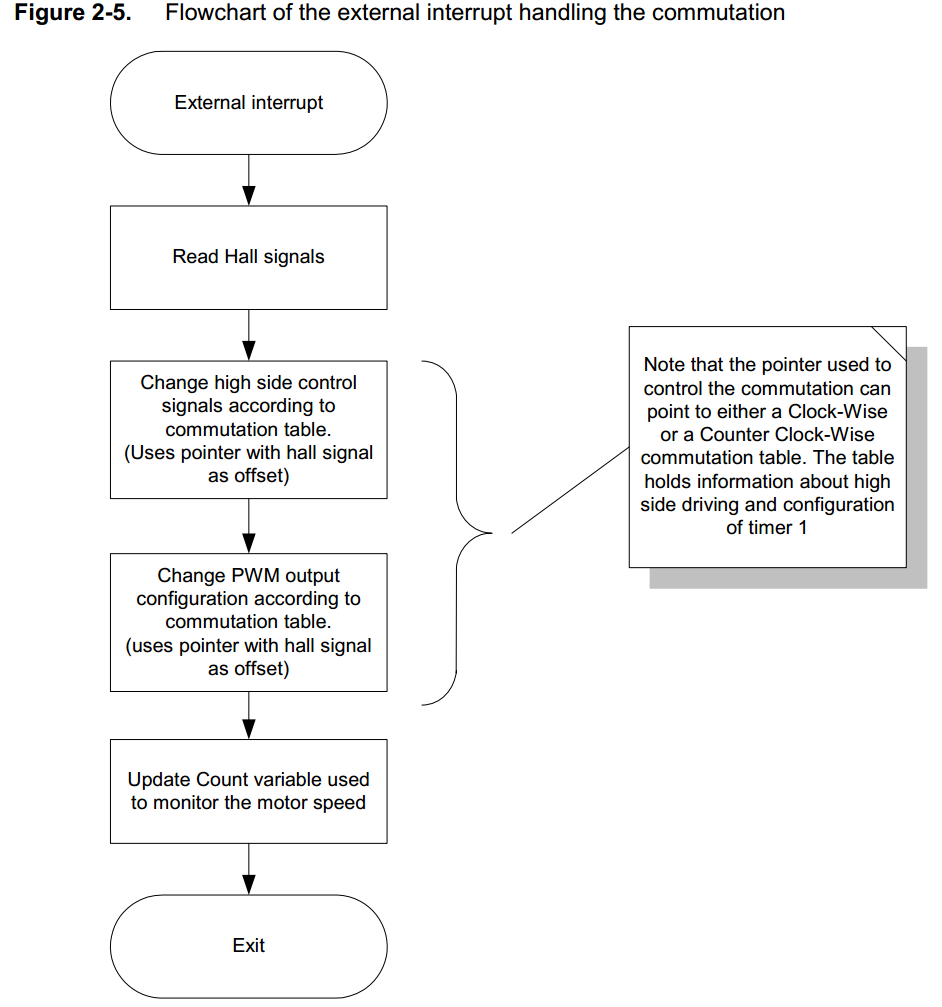
\includegraphics[width=\linewidth]{flowChart_hallInterrupt.png}

%=== END =======================================================================

\end{document}

